\documentclass[nobib]{tufte-handout}
\usepackage[utf8]{inputenc}
\usepackage[russian]{babel}

\usepackage{amsmath}
\usepackage{amsfonts}
\usepackage{amssymb}
\usepackage{url}
\usepackage{comment}
\usepackage[pdftex]{graphicx}
\usepackage{csquotes}
\usepackage{comment}
\usepackage{environ} % NewEnviron command
%\usepackage[left=2cm,right=2cm,top=2cm,bottom=2cm]{geometry}

\NewEnviron{solution}{%
    % \BODY
}%

\NewEnviron{problem}{%
    % \BODY
}%

\DeclareMathOperator{\Var}{Var}
\DeclareMathOperator{\Cov}{Var}
\DeclareMathOperator{\E}{E}


\usepackage{filecontents}



\begin{filecontents}{probability_dna.bib}
@book{феллер2013введение,
  title={Введение в теорию вероятностей и ее приложения},
  author={Феллер, Вильям},
  year={2010},
  publisher={URSS: Либроком},
  addendum={Очень старый и очень классный учебник по теории вероятностей в двух томах}
}

@book{секей2013парадоксы,
  title={Парадоксы в теории вероятностей и математической статистике},
  author={Секей, Габор},
  year={1990},
  publisher={Москва, Мир},
  addendum={Парадоксы с решениями и историей}
}

@article{winkler2002games,
  title={Games people don’t play},
  author={Winkler, Peter},
  journal={Puzzler’s Tribute: a Feast for the Mind},
  pages={301--313},
  url={http://www.teorver.ru/newkatalog/1193689162.pdf},
  year={2002},
  addendum={Несколько красивейших задач с решениями!}
}

@misc{gravner20problems,
  author={Gravner, Janko},
  title={Twenty problems in probability},
  url={https://www.math.ucdavis.edu/~gravner/MAT135A/resources/chpr.pdf}
}

@misc{kolmogorovolymps,
  title={Колмогоровские студенческие олимпиады по теории вероятностей},
  url={http://new.math.msu.su/department/probab/olimpia/olimpia.htm}
}


@misc{randompermutations,
  title={Свойства случайных перестановок},
  url={https://en.wikipedia.org/wiki/Random_permutation_statistics}
}


@book{blom1994problems,
  title={Problems and Snapshots from the World of Probability},
  author={Blom, Gunnar},
  year={1994},
  publisher={Springer},
  addendum={Задачи с решениями и небольшими исследованиями}
}

@article{ruggles1947empirical,
  title={An empirical approach to economic intelligence in World War II},
  author={Ruggles, Richard and Brodie, Henry},
  journal={Journal of the American Statistical Association},
  volume={42},
  number={237},
  pages={72--91},
  year={1947},
  publisher={Taylor \& Francis Group},
  addendum={Подробности про то, как имея всего два танка, можно оценить ежемесячный выпуск с точностью в пару процентов.}
}

@book{zade2003nevesta,
  title={Разборчивая невеста},
  author={Гусейн-Заде, С.М.},
  year={2003},
  publisher={МЦНМО},
  addendum={Задача в изложении для девятиклассников, \url{http://www.mccme.ru/mmmf-lectures/books/books/book.25.pdf}}
}

\end{filecontents}


\usepackage[sorting=none, backend=biber]{biblatex}
\addbibresource{probability_dna.bib}





\title{Теория вероятностей: культурный код}
\author{Фольклор}
\date{\today}
\begin{document}

\maketitle

\section{Культурный код}

Сборник восхитительных задач по элементарной теории вероятностей. Эти задачи --- наша вероятностная ДНК.

\section{Фольклор и красота}


\begin{enumerate}
\item Задача о Сумасшедшей Старушке.

\marginnote{Родилась она чисто из жизни --- а именно когда тогда еще юному автору приходилось часто ездить из Питера во Псков. Чаще всего билет на покупался в общий вагон поезда. На билете всегда было указано место. Но не тут-то было! Приходя в вагон, обнаруживалось, что пришедшие первыми занимали самые лучшие места (утверждая, что номера мест на билетах --- это просто для статистики). И вот тут-то и начинались эти цепочные сгоняния пассажиров.
В оригинале задачка звучала так: «В общем вагоне поезда Ленинград-Псков $N$ мест\ldots $N$-й пассажир, придя последним, обнаруживал, что свободно только только самое дурацкое место --- около туалета\ldots»  Но в редакции Кванта решили, что писать про бардак и туалет в общем вагоне поезда Лениград-Псков как-то не очень. И самовольно переделали условие на кинотеатр, \url{http://kvant.mccme.ru/1985/06/p34.htm}, автор: Игорь Алексеев}

В самолёте $100$ мест и все билеты проданы. Первой в очереди на посадку стоит Сумасшедшая Старушка. Сумасшедшая Старушка очень переживает, что ей не хватит места, врывается в самолёт и несмотря на номер по билету садиться на случайно выбираемое место. Каждый оставшийся пассажир садится на своё место, если оно свободно, и на случайное выбираемое место, если его место уже кем-то занято.

\begin{enumerate}
% \item Какова вероятность того, что все пассажиры сядут на свои места?
%\item Какова вероятность того, что второй пассажир в очереди сядет на своё место?
\item Какова вероятность того, что последний пассажир сядет на своё место?
\item Чему примерно равно среднее количество пассажиров севших на свои места?
\end{enumerate}

\begin{figure*}
  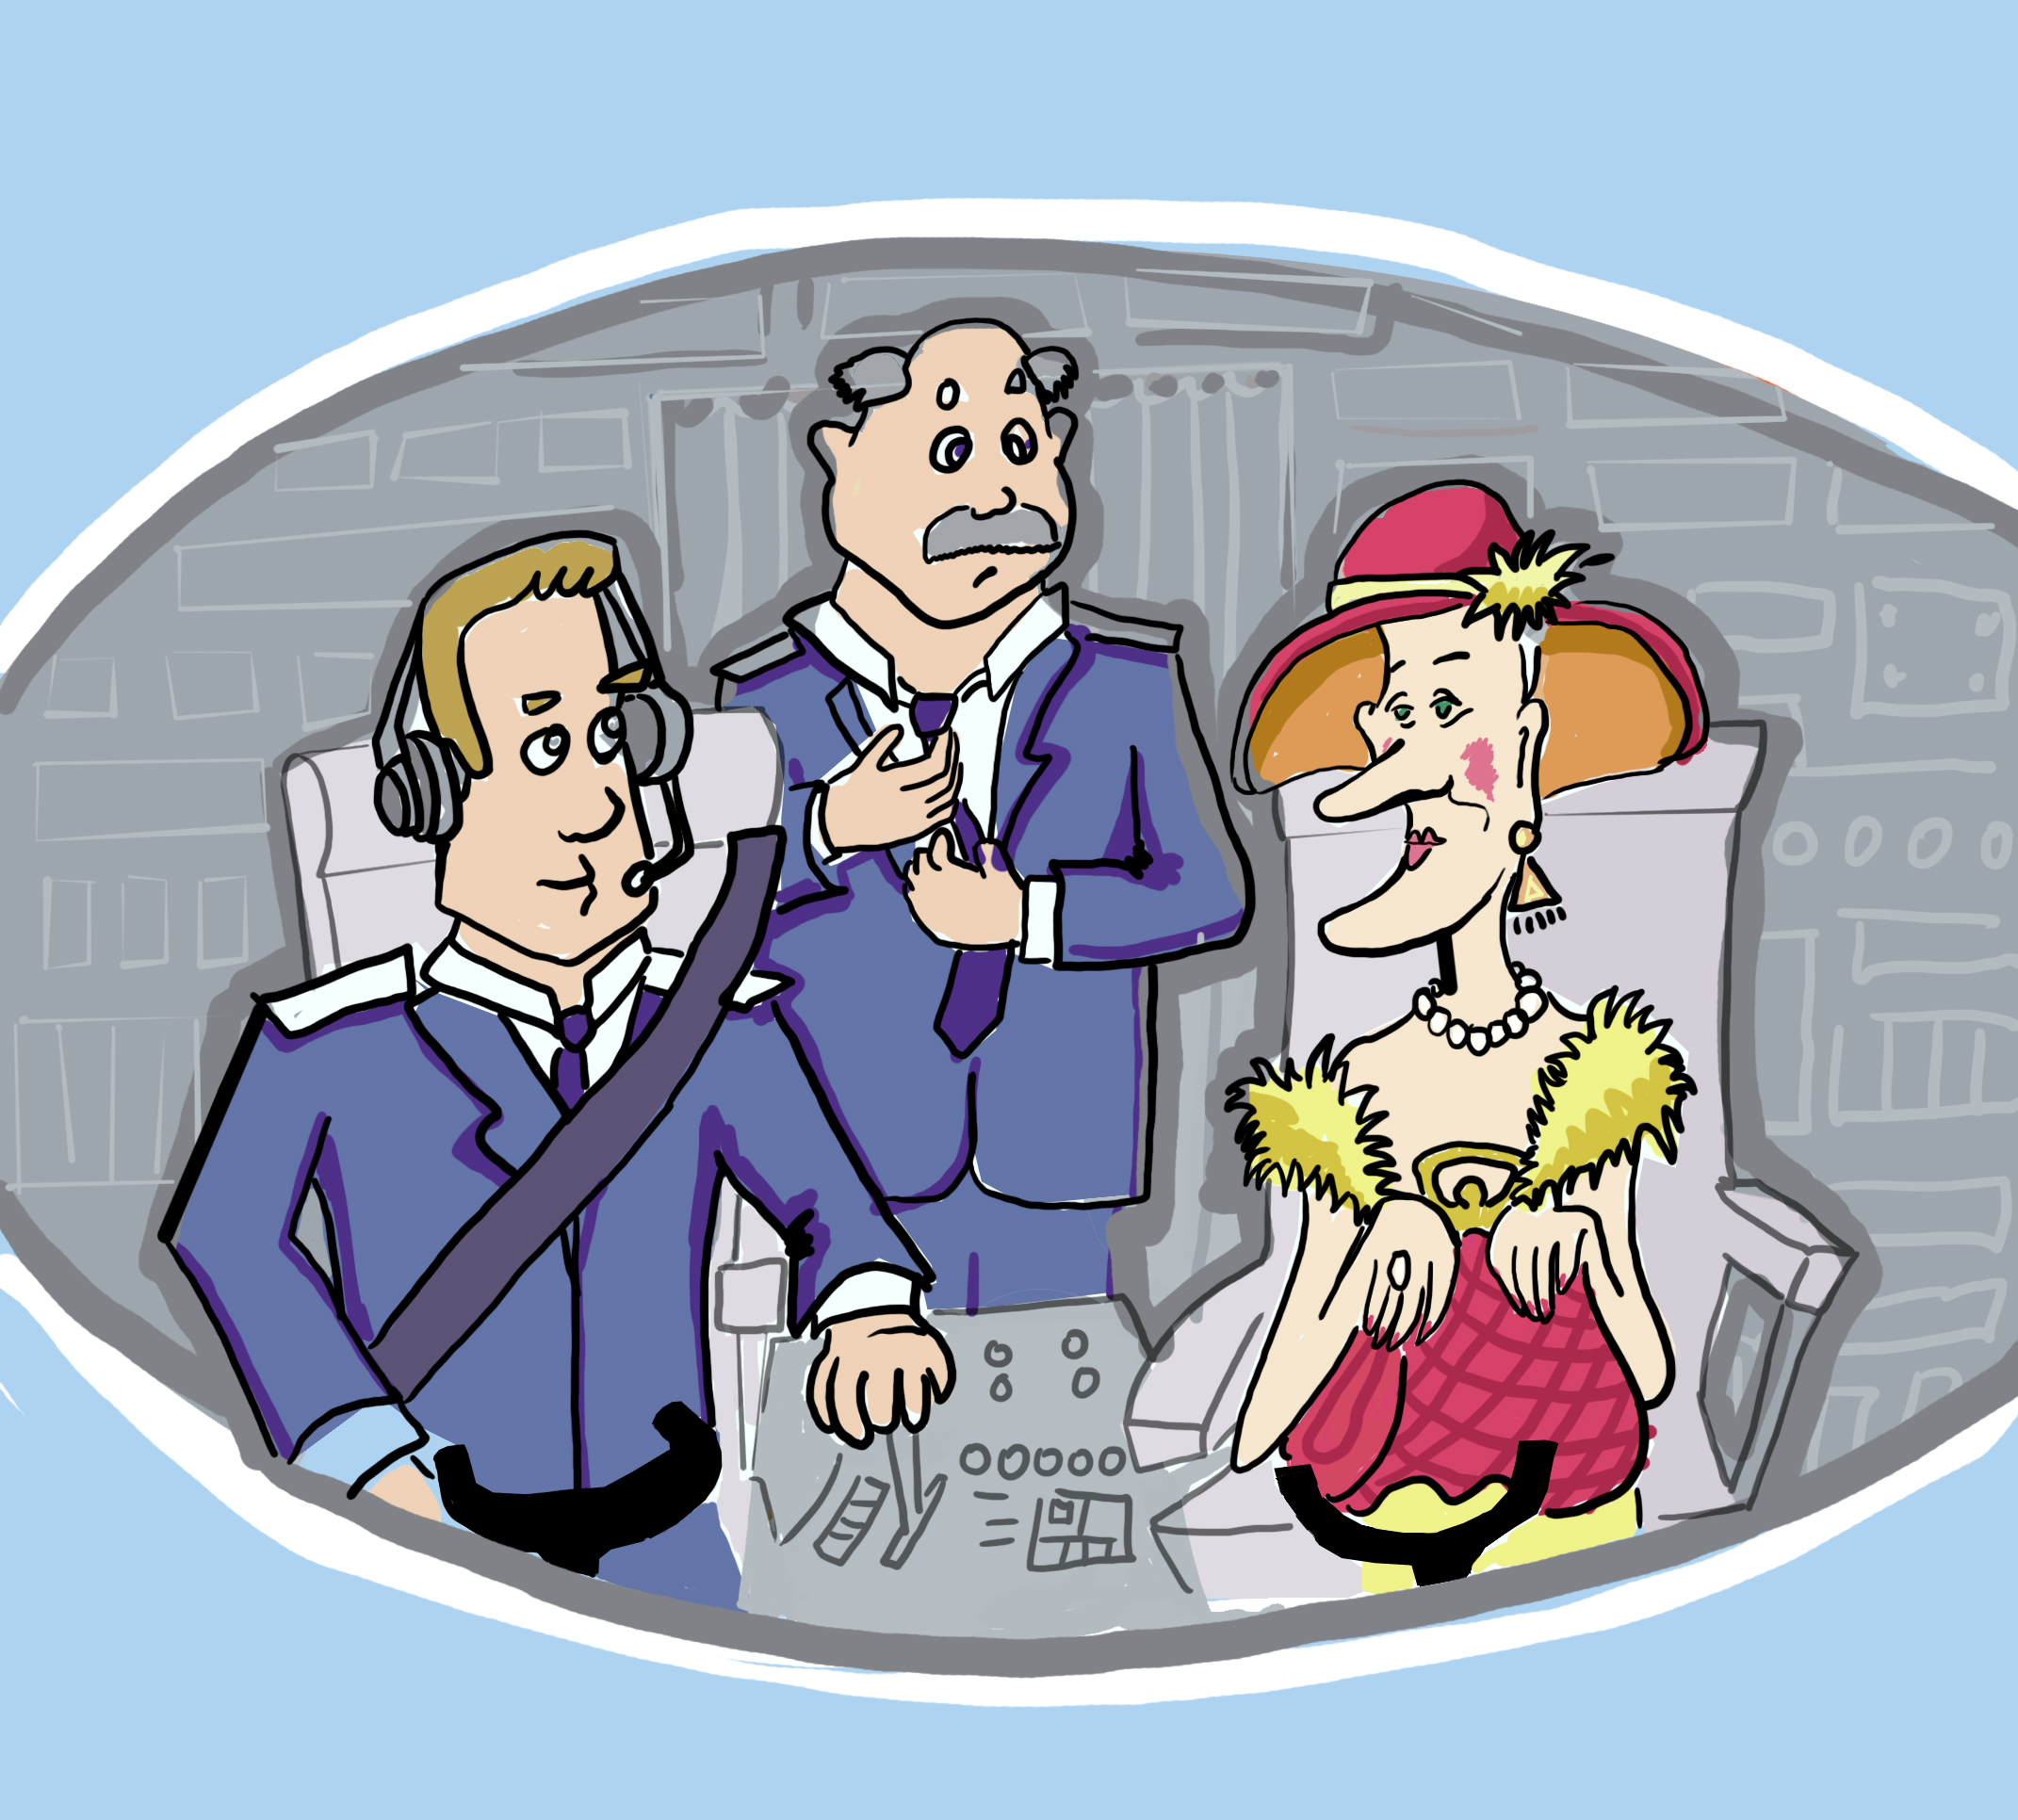
\includegraphics[width=17cm]{crazy_woman.jpg}
  \caption{--- Простите, пожалуйста, это место 1Б?}
\end{figure*}


\begin{solution}
Решение раз. Рассмотрим последовательность пересаживаний, начинающуюся с сумасшедшей старушки. В этой последовательности последний пассажир и сама сумасшедшая старушка равновероятно опережают друг друга. Следовательно, искомая вероятность равна $1/2$.

Решение два. Решаем задачу для $n=2$, $n=2$, получаем вероятность $1/2$. База индукции есть. Предположим, что для $1$, $2$, \ldots, $n-1$ пассажира вероятность равна $1/2$. В случае $n$ пассажиров первым ходом старушка может занять своё место, место последнего, какое-то другое место. Если она заняла своё, то последний точно сядет на своё место. Если она заняла место последнего, то он точно не сядет на своё место. Если она сядет на одно из оставшихся мест, то вскоре очередь дойдёт до того пассажира, чьё место она заняла. В этот момент можно считать, что он превратится в сумасшедшую старушку. Для меньшего количество пассажиров задача решена и даёт вероятность $1/2$. В силу симметрии получаем вероятность $1/2$ и для $n$ пассажиров.
\end{solution}

\item На самолёт, имеющий $100$ мест, проданы все билеты. Для посадки в
самолёт пассажиры выстроились в очередь. Первые 99 пассажиров "--- сумасшедшие старушки. Они садятся
на наугад выбранные места. Последний пассажир садится на то место,
которое указано в его билете. Если это место занято, то он с
помощью стюардессы сгоняет старушку со своего законного места.
Согнанная с чужого места сумасшедшая старушка становится
благоразумной и садится на свое место по билету. Возможно для
этого придется согнать еще одну старушку и т.д.
\begin{enumerate}
\item Какова вероятность того, что потревожат старушку, стоявшую $i$-ой в очереди?
\item Каково ожидаемое количество потревоженных старушек?
\end{enumerate}

\begin{solution}
\end{solution}

\item Задача собирателя наклеек. Coupon collector's problem.

Производитель чудо-юдо-йогуртов наклеивает на каждую упаковку одну из 50 случайно выбираемых наклеек. Покупатель собравший все виды наклеек получает приз от производителя. Пусть $X$ --- это количество упаковок йогурта, которое нужно купить, чтобы собрать все наклейки.

Найдите  $\E(X)$, $\Var(X)$

\begin{solution}
Количество наклеек можно разложить в сумму независимых случайных величин,
\[
X=Z_1+Z_2+\ldots+Z_n,
\]
где $Z_i$ --- количество наклеек, которые нужно докупить, чтобы найти $i$-ый новый вид наклейки, когда в коллекции уже есть наклейки $i-1$ вида. Конечно, $Z_1=1$.

Замечаем, что $\E(Z_i)=...$, $\Var(Z_i)=...$.
\end{solution}

\item Спички Банаха. Banach's matchbox problem.

Польский математик Стефан Банах имел привычку носить в каждом из двух карманов пальто по коробку спичек. Всякий раз, когда ему хотелось закурить трубку, он выбирал наугад один из коробков и доставал из него спичку. Первоначально в каждом коробке было по $n$ спичек. Но когда-то наступает момент, когда выбранный наугад коробок оказывается пустым.

\begin{enumerate}
\item Какова вероятность того, что в другом коробке в этот момент осталось ровно $k$ спичек?
\item Каково среднее количество спичек в другом коробке?
\end{enumerate}


\item Равновесие Харди-Вайнберга.

Предположим, что три возможных генотипа \verb|aa|, \verb|Aa| и \verb|AA| изначально встречаются с частотами $p_1$, $p_2$ и $p_3$, где $p_1+p_2+p_3=1$. Ген не сцеплен с полом, поэтому частоты $p_1$, $p_2$ и $p_3$ одинаковы для мужчин и для женщин.
\begin{enumerate}
\item У семейных пар из этой популяции рождаются дети. Назовём этих детей первым поколением. Каковы частоты для трёх возможных генотипов в первом поколении?
\item У семейных пар первого поколения тоже рождаются дети. Назовём этих детей вторым поколением. Каковы частоты для трёх возможных генотипов во втором поколении?
\item Каковы частоты для трёх возможных генотипов в $n$-ном поколении?
\item Заметив явную особенность предыдущего ответа сформулируйте теорему о равновесии Харди-Вайнберга. Прокомментируйте утверждение: «Любой рецессивный ген со временем исчезнет».
\end{enumerate}

\item Поляризация света.

Световая волна может быть разложена на две поляризованные составляющие, вертикальную и горизонтальную. Поэтому состояние отдельного поляризованного фотона может быть описано углом $\alpha$.\marginnote{На самом деле внутренний мир фотона гораздо разнообразнее.} Поляризационный фильтр описывается углом поворота $\theta$. Фотон в состоянии $\alpha$ задерживается поляризационным фильтром с параметром $\theta$ с вероятностью $p=\sin^2(\alpha-\theta)$ или проходит сквозь фильтр с вероятностью $1-p$, переходя при этом в состояние $\theta$.

\begin{enumerate}
\item Какова вероятность того, что поляризованный фотон в состоянии $\alpha$ пройдёт сквозь фильтр с параметром $\theta=0$?
\item Имеется два фильтра и поляризованный фотон в состоянии $\alpha$. Первый фильтр --- с $\theta=0$, второй --- c $\theta=\pi/2$. Какова вероятность того, что фотон пройдет через оба фильтра?
\item Имеется три фильтра и поляризованный фотон в состоянии $\alpha$. Первый фильтр --- с $\theta=0$, второй --- c $\theta=\beta$, третий --- с $\theta=\pi/2$. Какова вероятность того, что фотон пройдет через все три фильтра? При каких $\alpha$ и $\beta$ она будет максимальной и чему при этом она будет равна?\marginnote{Как сделать «секретный монитор» своими руками, \url{http://www.youtube.com/watch?v=-ojbykV1zyc}}
\item Объясните следующий фокус. Фокусник берет два специальных стекла и видно, что свет сквозь них не проходит. Фокусник ставит между двумя стёклами третье, и свет начинает проходить через три стекла.
\end{enumerate}


\item Истеричная певица

Начинающая певица дает концерты каждый день. Каждый ее концерт приносит продюсеру 0.75 тысяч евро. После каждого концерта певица может впасть в депрессию с вероятностью 0.5. Самостоятельно выйти из депрессии певица не может. В депрессии она не в состоянии проводить концерты. Помочь ей могут только цветы от продюсера. Если подарить цветы на сумму $0\le x\le 1$ тысяч евро, то она выйдет из депрессии с вероятностью $\sqrt{x}$.

Какова оптимальная стратегия продюсера?

\item Парадокс Симпсона.  Simpson's Paradox.

Два лекарства испытывали на мужчинах и женщинах. Каждый
человек принимал только одно лекарство. Общий процент людей,
почувствовавших улучшение, больше среди принимавших лекарство А.
Процент мужчин, почувствовавших улучшение, больше среди мужчин, принимавших лекарство В. Процент женщин, почувствовавших улучшение, больше среди женщин, принимавших лекарство В.

\begin{enumerate}
\item Возможно ли это?
\item Какое лекарство нужно посоветовать принять пациенту, если его пол неизвестен?
\end{enumerate}


\item Вовочку перевели из класса А в класс Б. Мог ли при этом возрасти средний балл по математике в обоих классах?

\begin{solution}
Да, возможно, если уровень Вовочки ниже среднего уровня класса А, но выше среднего уровня класса Б.
\end{solution}

\begin{figure*}
  
\includegraphics[width=17cm]{average.png}
  \caption{Dilbert}
\end{figure*}



\item Злобный дракон поймал трех гномов. И решил поиграться с ними. Каждому гному он надевает с равными вероятностями черный или белый колпак.
\marginnote{ --- Значит, дракон --- это датчик случайных колпаков?}


Гномы видят чужие колпаки, но не видят своих и не могут общаться после выдачи колпаков. Каждый гном может попытаться угадать цвет своего колпака, либо промолчать. Дракон отпустит гномов, если хотя бы один гном угадал цвет своего колпака, и никто не сделал ошибки. Если все одновременно промолчали, или кто-нибудь ошибся, то все гномы будут съедены. Перед игрой гномы могут договориться о стратегии игры.
\begin{enumerate}
\item Как гномам следует играть, если Злобный дракон спрашивает их по очереди? Какова вероятность того, что они будут спасены?
\item Как гномам следует играть, если они должны дать ответ одновременно? Какова вероятность того, что они будут спасены?
\item Если от далекого спутника нужно получить один бит информации («да» или «нет»), то, отправив три бита, можно не бояться того, что природа «испортит» один из них. Постройте этот простой код. Проведите аналогию с предыдущим пунктом. \marginnote{ --- Три гнома --- три бита?}
\end{enumerate}
Идея этой задачи используется не только при космической связи. Чтобы неглубокие царапины на компакт диске не вызывали потерь данных, при записи используется код Рида-Соломона.
\marginnote{ --- А как звали третьего гнома?}

\item Париж, Людовик XIV, 1654 год, высшее общество говорит о рождении новой науки --- теории вероятностей. Ах, кавалер де Мере, «fort honnête homme sans être mathématicien»\ldots \marginnote{«благородный человек, хотя и не математик».} Старая задача, неправильные решения которой предлагались тысячелетиями (например, одно из неправильных решений предлагал изобретатель двойной записи, кумир бухгалтеров, Лука Пачоли) наконец решена правильно!


Два игрока играют в честную игру до шести побед. Игрок первым выигравший шесть партий (не обязательно подряд) получает 800 луидоров. К текущему моменту первый игрок выиграл 5 партий, а второй --- 3 партии. Они вынуждены прервать игру в данной ситуации.


Как им поделить приз по справедливости?

\begin{center}
\begin{figure*}[t]
  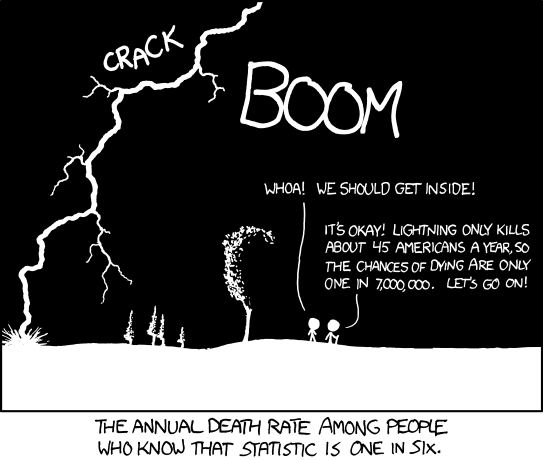
\includegraphics[width=10cm]{conditional.png}
  \caption{\url{http://xkcd.com/795/}}
\end{figure*}
\end{center}

\item На арене две команды гладиаторов,  $A$  и  $B$ . Каждый гладиатор обладает определенной силой, неизменной по ходу игры. Команды могут отличаться по количеству гладиаторов и их силе. Игра проходит в виде последовательных турниров, в каждом из которых участвует по одному гладиатору от каждой стороны. Если в очередном турнире встречаются гладиаторы с силами  $a$  и  $b$ , то вероятность победы первого определяется величиной  $\frac{a}{a+b} $ . Гладиатор, проигравший турнир, выбывает из игры, выигравший --- возвращается в команду. Гладиаторы не устают, но и не приобретают опыта. Стратегия команды предписывает, какого гладиатора выдвигать на очередной турнир в зависимости текущего состава команд. Игра ведется до полного выбывания из игры одной из команд.

Как выглядит оптимальная стратегия команды $A$?

\item В отличие от обычного гладиатора, у победившего гладиатора-вампира сила увеличивается на силу побежденного им гладиатора-вампира. В остальном правила поединка такие же, как в предыдущей задаче.

Как выглядит оптимальная стратегия команды $A$?

\item Маша и Саша играют в быстрые шахматы. У них одинаковый класс игры и оба предпочитают играть белыми, т.е. вероятность выигрыша белых  $p>0.5$. Партии играются до 10 побед. Первую партию Маша играет белыми. Она считает, что в следующей партии белыми должен играть тот, кто выиграл предыдущую партию. Саша считает, что ходить белыми нужно по очереди. При каком варианте правил у Маши больше шансы выиграть?

\item Гадалка

Маша пишет на бумажках два любых различных натуральных числа по своему выбору. Одну бумажку она прячет в левую руку, а другую --- в правую. Саша выбирает любую Машину руку. Маша показывает число, написанное на выбранной бумажке. Саша высказывает свою догадку о том, открыл ли он большее из двух чисел или меньшее. Если Саша не угадал, то Маша выиграла.

Существует ли у Саши стратегия, гарантирующая ему выигрыш с вероятностью строго более 50\%, даже будучи известной Маше?

\begin{figure*}
  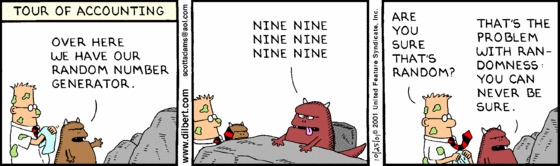
\includegraphics[width=17cm]{ninenine.png}
  \caption{Dilbert, «We guarantee that each number is random individually, but we don't guarantee that more than one of them is random», \url{http://en.wikipedia.org/wiki/RANDU}}
\end{figure*}


\item Больший кусок окружности

Аня хватается за верёвку в форму окружности в произвольной точке. Боря берёт мачете и с завязанными глазами разрубает верёвку в двух случайных независимых местах. Аня забирает себе тот кусок, за который держится. Боря забирает оставшийся кусок.  Вся верёвка имеет единичную длину.
\begin{enumerate}
\item Чему равен ожидаемый длина куска верёвки, доставшегося Ане?
\item  Вероятность того, что у Ани верёвка длиннее?
\end{enumerate}


\item Судьба Дон-Жуана.

У Дон-Жуана $n$  знакомых девушек, и их всех зовут по-разному. Он пишет
им $n$  писем, но по рассеянности раскладывает их в конверты
наугад. Случайная величина $X$ обозначает количество девушек, получивших письма, адресованные лично им.

\begin{enumerate}
\item Найдите $\E(X)$, $\Var(X)$
\item Какова при большом $n$ вероятность того, что хотя бы одна девушка получит письмо, адресованное ей?
\end{enumerate}



\item Ефросинья подкидывают правильную монетку неограниченное количество раз.

\begin{enumerate}
\item Сколько в среднем нужно сделать бросков до появления последовательности ОРОР? До появления последовательности РОРР?
\item Какова вероятность того, что ОРОР появится раньше РОРР?
\item Какова вероятность того, что ООО появится позже РРОО?
\item Каковы вероятности того, что ООР появится раньше ОРР? ОРР раньше РРО? РРО раньше РОО? РОО раньше ООР?
\end{enumerate}

\item Илье Муромцу предстоит дорога к камню. От камня начинаются ещё три дороги. Каждая из тех дорог снова оканчивается камнем. И от каждого камня начинаются ещё три дороги. И каждые те три дороги оканчиваются камнем\ldots И так далее до бесконечности. На каждой дороге живёт трёхголовый Змей Горыныч. Каждый Змей Горыныч бодрствует независимо от других с вероятностью (хм, Вы не поверите!) одна третья. У Василисы Премудрой существует Чудо-Карта, на которой видно, какие Змеи Горынычи бодрствуют, а какие --- нет. Какова вероятность того, что Василиса Премудрая сможет найти на карте  бесконечный жизненный путь Ильи Муромца проходящий исключительно мимо спящих Змеев Горынычей?

\item У тети Маши --- двое детей разных возрастов. Вероятности рождения мальчика и девочки равны.

\begin{enumerate}
\item Какова вероятность того, что у тёти Маши оба ребёнка --- мальчики, если известно, что у неё хотя бы один ребёнок --- мальчик?
\item Какова вероятность того, что у тёти Маши оба ребёнка --- мальчики, если известно, что у неё хотя бы один ребёнок --- мальчик водолей по гороскопу?
\end{enumerate}

\item Buffon's needle problem

Плоскость разлинована параллельными линиями через каждый сантиметр. Случайным образом на эту плоскость бросается иголка длины $a<1$.

\begin{enumerate}
\item Какова вероятность того, что иголка пересечёт какую-нибудь линию?
\item Предложите вероятностный способ оценки числа $\pi$
\end{enumerate}

\begin{solution}
Поскольку $a<1$ количество пересечений равно либо 0, либо 1, следовательно, вероятность пересечения равна математическому ожиданию числа пересечений. Обозначим $X$ --- количество пересечений. Если иголку удлиннить в $n$ раз, то $\E(X)$ изменится в $n$ раз, так как фактически мы имеем $n$ иголок равной длинны. Если иголку согнуть в ломаную, то $\E(X)$ не меняется, так как снова иголка разрезается на отдельные иголки. Отсюда получаем, что $\E(X)$ зависит только от длины иголки, но не от формы. Сгибаем иголку в окружность. Если длина равна $\pi$, то пересечений будет два. Значит при длине $a$ ожидаемое количество пересечений равно $2a/\pi$.
\end{solution}



\item Мартышка и Шекспир

Мартышка наугад нажимает клавиши на печатающей машинке.


\begin{enumerate}
\item Какова вероятность того, что она рано или поздно напечатает полное собрание сочинений Шекспира? Льва Толстого?
\item Обозначим количество нажатий до появления слова «АБРАКАДАБРА» за $X$. Найдите $\E(X)$ и $\Var(X)$.
\end{enumerate}


\begin{marginfigure}
  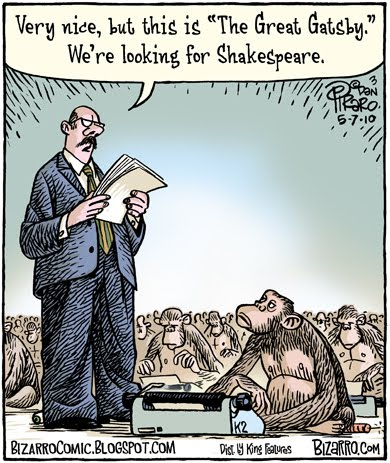
\includegraphics[width=5cm]{gatsby}
  \caption{Задача о «бесконечных обезьянах», infinte-monkey problem. }
\end{marginfigure}

\item Парадокс инспектора

Автобусы приходят на остановку согласно пуассоновскому потоку в среднем один раз в час. Вася приходит на остановку в случайный момент времени и садится на первый пришедший автобус.

\begin{enumerate}
\item Сколько Васе в среднем предстоит ждать автобуса?
\item Сколько в среднем прошло времени от последнего пришедшего автобуса до Васиного появления?
\item Чему равна средняя продолжительность интервала между автобусом, на который сядет Вася, и предыдущим?
\item Чему равна средняя продолжительность интервала между автобусом, на который сядет Вася, и следующим?
\item Маша не любит набитые битком автобусы и никогда не торопится, поэтому, придя на остановку, всегда пропускает один автобус и садится на следующий. Она считает, что на него в среднем сядет меньше людей. Права ли она?
\end{enumerate}


\begin{solution}
Да, Маша права, на «следующий» в среднем садиться меньше пассажиров.
\end{solution}


\item Спящая красавица

Спящая красавица согласилась принять участие в научном
эксперименте. В воскресенье её специально уколют веретеном. Как
только она заснёт, будет подброшена правильная монетка.


Если
монетка выпадет орлом, то спящую красавицу разбудят в понедельник
и спросят о том, как выпала монетка.


Если монетка выпадет решкой,
то спящую царевну разбудят в понедельник, спросят о монетке, снова
уколют веретеном, разбудят во вторник и снова спросят о монетке.
Укол веретена вызывает легкую амнезию, и красавица не сможет
определить, просыпается ли она в первый раз или во второй.


Красавица только-только проснулась. Вспомнила правила эксперимента, и услышала вопрос исследователя: «Ваше Высочество, так как же выпала монетка?»
\begin{enumerate}
\item Как следует отвечать красавице, если за каждый верный ответ ей
дарят молодильное яблоко?
\item Как следует отвечать красавице, если за неверный ответ её тут
же превращают в тыкву?
\item Отвечая на вопрос исследователя Спящая Красавица задумалась, а какова вероятность того, что сегодня понедельник. Как ты думаешь?
\end{enumerate}



\begin{solution}
«Сегодня понедельник» "--- это \textbf{не} событие. Вероятность не
определена. Это функция от времени.

Вероятность того, что монетка выпала орлом, равна $0{,}5$. Поэтому ей
всё равно, как отвечать, если наказанием является превращение в
тыкву, и нужно отвечать: «Решка!» "--- если наградой является
молодильное яблоко. Предположим, что красавица максимизирует
ожидаемое количество молодильных яблок.
\end{solution}

\item Monty-Hall

Есть три закрытых двери. За двумя из них --- по козе, за третьей автомобиль. Вы выбираете одну из дверей. Допустим, Вы выбрали дверь А. Ведущий шоу, чтобы поддержать интригу, не открывает сразу выбранную Вами дверь. Сначала он открывает одну из дверей не выбранных Вами, причем снова ради интриги ведущий не открывает сразу и дверь с автомобилем. Допустим, ведущий открыл дверь B. И в этот момент он предлагает Вам изменить ваш выбор двери.

Имеет ли смысл изменить свой выбор?

\begin{figure*}
  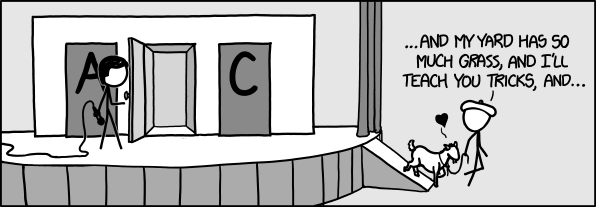
\includegraphics[width=17cm]{monty_hall}
  \caption{A few minutes later, the goat from behind door C drives away in the car. \url{http://xkcd.com/1282/}}
\end{figure*}


\item Monty-Hall версия

Трое студентов, Аня, Боря и Василиса, сдавали комиссию по теории вероятностей и ещё не знают своих оценок. Им объявили, что зачёт получили двое из трёх. В перерыве перед объявлением оценок Боря подходит к председателю:

--- Иван Иванович, раз зачёт получили двое из трёх, значит хотя бы у одной из девушек есть зачёт. Вы мне можете назвать имя одной из девушек, получившей зачет?

--- Василиса получила.

Какова условная вероятность того, что Боря получил зачёт, если принимать во внимание информацию от Ивана Ивановича?

\item Задача о Разборчивой Невесте, Secretary problem

К Разборчивой невесте выстроилась вереница из $n»0$ потенциальных женихов.  \marginnote{Докторская диссертация член-корреспондента РАН Бориса Березовского «Разработка теоретических основ алгоритмизации принятия предпроектных решений и их применения»  является обобщением задачи о разборчивой невесте, \url{http://en.wikipedia.org/wiki/Secretary_problem}} Разборчивая невеста хочет выбрать самого богатого из них и только его! Потенциальные женихи заходят к Разборчивой невесте по одному в случайном порядке. Невеста неплохо разбирается в богатстве и всегда может ранжировать всех, с кем она общалась, по величине богатства. Когда к Разборчивой невесте приходит очередной претендент, она должна сразу принять решение: выбрать данного кандидата или перейти к следующему. Вернуться к предыдущим кандидатам невозможно --- они обижаются и уезжают.

\begin{enumerate}
\item Как выглядит оптимальная стратегия Разборчивой невесты? Чему равна вероятность выбора самого богатого жениха Разборчивой невестой?
\item Подруга-дурнушка Разборчивой невесты хочет выбрать второго по богатству жениха и только его! \marginnote{Всё равно самый богатый достанется Разборчивой невесте!} Как выглядит её оптимальная стратегия? Чему равна вероятность выбора второго по богатству жениха Подругой-дурнушкой?
\end{enumerate}

\item Собрались $n»0$ ковбоев. Каждый из них выбрал себе из остальных своего самого главного врага случайным образом. Далее ковбои по очереди стреляют, каждый в своего главного врага. Естественно, если жив сам, и если жив самый главный враг. Ковбои стреляют без промаха.
\begin{enumerate}
\item Какая доля ковбоев в среднем останется в живых?
\item Какая доля ковбоев в среднем останется в живых, если треть ковбоев забыла дома свой кольт?
\end{enumerate}

\item Задача Бертрана о голосовании, Betrand's ballot theorem

За кандидата А было подано 100 голосов, а за кандидата Б --- 300 голосов.
\begin{enumerate}
\item Какова вероятность того, что во время голосования постоянно лидировал кандидат Б?
\item Какова вероятность того, что во время всего голосования за кандидата А  голосов было больше, чем в два раза, чем за кандидата Б?
\end{enumerate}

\url{http://en.wikipedia.org/wiki/Bertrand%27s_ballot_theorem}

\url{http://webspace.ship.edu/msrenault/ballotproblem/monthly358-363-renault.pdf}


\item Задача о макаронах

В тарелке запутавшись лежат $n>>0$ макаронин. Я по очереди связываю попарно все торчащие концы макаронин.

\begin{enumerate}
\item Какова примерно вероятность того, что я свяжу все макаронины в одно большое кольцо?
\item Сколько в среднем колец образуется?
\item Каково среднее число колец длиной в одну макаронину?
\end{enumerate}

\item Задача о ключах и копилках

На столе стоят $n$ свиней-копилок. Достать содержимое копилки можно двумя
способами: либо разбить копилку, либо открыть дно специальным
ключиком. К каждой копилке подходит единственный ключ. Мы раскладываем ключи по
копилкам наугад, один ключ в одну копилку. Затем разбиваем $k$ копилок и получаем хранящиеся в них ключи. Далее мы будем копилки только открывать ключами.
\begin{enumerate}
\item Какова вероятность того, что мы сможем достать все ключи?
\item Какая доля ключей в среднем будет найдена?
\end{enumerate}


\item Парадокс двух конвертов. Two envelope paradox

Перед тобой два внешне одинаковых конверта. В одном из них лежит ровно в два раза больше денег, чем в другом. Ты открываешь один из конвертов и видишь, что в нём лежит $x$ рублей. У тебя есть возможность взять открытый конверт или отказаться от него и взять сумму в закрытом конверте.

\begin{enumerate}
\item Чему равно математическое ожидание суммы денег, лежащей в закрытом конверте?
\item Какой конверт стоит предпочесть, уже открытый или еще закрытый?
\item Предположим, что деньги в конверты кладут следующим образом: в один из конвертов кладут случайную сумму денег, имеющую экспоненциальное распределение с параметром $\lambda=1$, а в другой конверт --- в два раза больше. Как выглядит оптимальная стратегия игрока?
\item Предположим, что деньги в конверты кладут другим образом. Сначала подбрасывают правильную монетку до тех пор, пока не выпадет «орёл». Обозначим количество подбрасываний буквой $N$. В один из конвертов кладут $3^N$ рублей, а в другой конверт --- в три раза больше. Как выглядит оптимальная стратегия игрока?
\end{enumerate}


\item Удвоение ставки

Два игрока играют в справедливую игру. Позицию в игре в момент времени $t$ условно можно описать числом $p_t \in [0;1]$, вероятностью победы первого игрока. Время непрерывно. Изначально $p_0=1/2$. Величина $p_t$ ведёт себя как броуновское движение. Игра оканчивается, когда $p_t$ достигает $0$ или $1$.

Игрок владеющий красной меткой в любой момент игры может предложить другому удвоить ставки. Изначально красная метка находится у первого игрока. После удвоения ставок красная метка переходит к другому игроку.

В какой момент следует предлагать удвоение ставок?

\item Есть три рулетки: \marginnote{Кто первый встал, того и тапки!} на первой равновероятно выпадают числа 2, 4 и 9; на второй --- 1, 6 и 8; на третьей --- 3, 5 и 7. Сначала первый игрок выбирает рулетку себе, затем второй игрок выбирает рулетку себе из двух оставшихся. После этого рулетки, выбранные игроками, запускаются, и случай определяет победителя. Победителем считается тот, чья рулетка покажет большее число. \marginnote{Первой пташке достается червячок, но сыр съедает вторая мышка.}

\begin{enumerate}
\item В чью пользу эта игра?
\item Какая рулетка самая хорошая?
\end{enumerate}

\item На европейской рулетке 18 черных ячеек, 18 красных ячеек и одно зелёное зеро. Васиссуалий приходит в казино имея 100 рублей денег. Он ставит на чёрное по одному рублю до тех пор, пока не проиграет все деньги или его благосостояние не достигнет 200 рублей.

\begin{enumerate}
\item Какова вероятность того, что Васиссуалий покинет казино имея 200 рублей?
\item Как изменится ответ, если Васиссуалий играет в американскую рулетку, на которой помимо одинарного зеро есть и двойное зеро?
\end{enumerate}

\item Санкт-Петербургский парадокс

Тебе предлагают сыграть в следующую игру. Правильную монетку подкидывают до первого выпадения «орла». Если впервые «орёл» выпадает при $N$-ом подбрасывании, то ты получаешь $2^N$ рублей.

\begin{enumerate}
\item Чему равно математическое ожидание выигрыша в эту игру?
\item Сколько ты согласен заплатить за однократное участие в этой игре?
\end{enumerate}

\begin{solution}
Математическое ожидание выигрыша равно бесконечности:
\[
\frac{1}{2}\cdot 2 + \frac{1}{2^2}\cdot 2^2 + \frac{1}{2^3}\cdot 2^3 + \ldots = +\infty
\]
Оплата за однократное участие --- субъективна.
\end{solution}

\item Труэль

Три игрока решили стреляться ради самой красивой девушки и организуют труэль (дуэль для трёх игроков).  Игроки стреляют по очереди, $A$-$B$-$C$-$A$-\ldots. Каждый из игроков может либо целиться в одного из противников, либо стрелять в воздух. Вероятности попадания равны $p_a=0.6$, $p_b=0.5$ и $p_c=0.4$, соответственно. Игра продолжается до определения единственного победителя, он и получает девушку в жёны.

\begin{enumerate}
\item Как выглядит оптимальная стратегия каждого игрока?
\item Чему равные вероятности выиграть для каждого игрока?
\end{enumerate}



\item Игра Паррондо

В игре $A$ ты с вероятностью $0.45$ выигрываешь один рубль и с вероятностью $0.55$ проигрываешь один рубль.

Игра $B$ чуть более хитрая. Если сумма в твоём кошельке делится на три, то ты выигрываешь один рубль с вероятностью $0.05$ и проигрываешь один рубль с вероятностью $0.95$. Если же
сумма в твоем кошельке не делится на три, то ты выигрываешь один рубль с вероятностью $0.7$ и проигрываешь один рубль с вероятностью $0.3$.

Изначально у тебя в кошельке 100 рублей. Что произойдёт с твоим благосостоянием, если:

\begin{enumerate}
\item Ты будешь бесконечное количество раз играть в игру $A$?
\item Ты будешь бесконечное количество раз играть в игру $B$?
\item Ты будешь бесконечное количество раз равновероятно выбирать игру $A$ или игру $B$?
\end{enumerate}



\item Во время Второй Мировой войны американские военные собрали статистику попаданий пуль в фюзеляж самолёта.  По самолётам, вернувшимся из полёта на базу, была составлена карта повреждений среднестатистического самолёта. С этими данными военные обратились к статистику Абрахаму Вальду с вопросом, в каких местах следует увеличить броню самолёта.

Что посоветовал Абрахам Вальд и почему?

\begin{solution}
На базу будут возвращаться только самолёты, имеющие некритичные повреждения. Поэтому чем больше попаданий в какое-то место самолёта, тем менее данное место важно для живучести самолёта. Абрахам Вальд посоветовал укреплять те места, где не было попаданий.
\end{solution}

\item Задача о немецких танках
\marginnote{Незадолго до высадки союзников в Нормандии, 6 июня 1944 года, в распоряжении союзников было всего два (!) немецких танка «Пантера V». По серийным номерам на шасси танков союзники оценили выпуск в феврале 1944 в 270 танков. Фактический выпуск «Пантер V» согласно немецким документам в феврале 1944 составил 276 танков, \autocite{ruggles1947empirical}. }

Предположим, что все выпущенные танки имеют порядковый номер. От самого первого выпущенного танка, имеющего номер $1$, до самого последнего танка, имеющего номер $n$. В бою удалось подбить танки с номерами $15$, $29$ и $23$.

\begin{enumerate}
\item Постройте оценку количества танков методом моментов
\item Постройте оценку количества танков методом максимального правдоподобия
\item Постройте несмещенную оценку количества танков с наименьшей дисперсией
\end{enumerate}

\begin{solution}
Оценка метода моментов:
\[
\hat{n}_{MM}=2\bar{X}-1
\]
Оценка максимального правдоподобия:
\[
\hat{n}_{ML}=\max\{X_1,X_2, \ldots, X_k\}
\]

\end{solution}

\item Саша и Маша хорошо перетасовали колоду в 52 карты и удалили из неё все онёры («картинки»), так что остались одни фоски (числовые карты). Саша выбирает одну из первых 10 карт наугад. Узнав значение этой карты, он открывает соответствующую следующую по счёту карту. Открыв новую карту и руководствуясь её значением, Саша открывает еще одну новую карту и т.д. до тех пор, пока хватает колоды.

Не перемешивая колоду Маша повторяет Сашин алгоритм действий. С помощью симуляций определите, какова примерно вероятность того, что Саша и Маша остановятся на одной карте.

\item Парчовую ленту длиной 1 км разрезают в $(n-1)$-ом случайно равномерно распределенном месте, чтобы поделить её на $n$ принцесс. Скромнице Василисе достаётся самый короткий кусочек ленты.

\begin{enumerate}
\item Какова ожидаемая длина Василисиного куска?
\item Какова ожидаемая длина самого короткого кусочка кроме Василисиного?
\end{enumerate}

\begin{solution}
Найдём вероятность того, что минимальная длина больше $d$. Представим себе большую колоду из $N$ карт, в которой $(n-1)$ отмеченная карта. Нам нужна вероятность того, что при вытягивании карт по очереди между ними будет минимум $dN$ карт. Однако при вытягивании меченой карты, можно следующие $dN$ карт вытягивать с конца колоды. Это не повлияет на случайность порядка, а вероятность будет считать проще. Нам нужна фактически вероятность того, что в конце колоды будет $(n-1)dN$ немеченных карт и $dN$ немеченных карт в начале колоды.


В случае $k$-го по счёту минимального куска:
\[
\frac{1}{n}\left( \frac{1}{n} + \ldots + \frac{1}{k}\right)
\]

Идея доказательства:
\[
\E(X) + \frac{1-n\E(X)}{(n-1)^2}=\ldots=\frac{1}{n}\left( \frac{1}{n} + \frac{1}{n-1}\right)
\]
\end{solution}


\item  Роковая дама играет в азартную игру. Перед дамой хорошо перетасованная колода в 52 карты. Дама открывает карты одну за одной. В любой момент дама может сделать пророчество «Следующая карта будет дамой». Если пророчество сбывается, то дама получает 100 рублей.

\begin{enumerate}
\item Какова оптимальная стратегия дамы?
\item Какова вероятность выигрыша при использовании оптимальной стратегии?
\end{enumerate}

\begin{solution}
Вместо того, чтобы делать ставку на следующую карту, можно делать ставку на последнюю карту, т.к. информация о них одинаковая. А для последней карты не важно, когда делать пророчество, поэтому все стратегии приносят вероятность выигрыша $4/52$.
\end{solution}

\item Ветреная Машенька пишет романтические смс Андрею и Борису. Первое смс она пишет Андрею, второе --- Борису и третье --- Борису. Далее каждое следующее смс она пишет Андрею с вероятностью равной доле ранее отправленных Андрею смс. Всего за день Машенька отправила 100 смс.

\begin{enumerate}
\item Какова вероятность того, что четвёртое смс она напишет Борису?
\item Какова вероятность того, что 100-ое смс она напишет написано Борису?
\item Какова вероятность того, что последние три смс она напишет Борису?
\item Сколько в среднем смс она напишет Борису?
\item Какова вероятность того, что ровно 20 смс она напишет Борису?
\item Какова вероятность того, что ровно $k$ смс она напишет Борису?
\item Машенька продолжает писать смс Андрею и Борису, не остановившись на $n=100$. Она загадала, что если тысячу раз подряд напишет смс Борису, то выйдет за него замуж. Какова вероятность, того, что Машенька выйдет замуж за Бориса? Сколько в среднем смс всего до замужества она напишет?
\end{enumerate}

\begin{solution}


\end{solution}

\item Злобный Дракон поймал принцесс Настю и Сашу и посадил в разные башни. Перед каждой из принцесс Злобный Дракон подбрасывает один раз правильную монетку. А дальше даёт каждой из них шанс угадать, как выпала монетка у её подруги. Если хотя бы одна из принцесс угадает, то Злобный Дракон отпустит принцесс на волю. Если обе принцессы ошибутся, то они навсегда останутся у него в заточении.

Подобная практика у Злобного Дракона исследователями была отмечена уже давно, поэтому принцессы имели достаточно времени договориться на случай вероятного похищения.

Как следует поступать принцессам при подобных похищениях?

\begin{solution}
Настя может угадывать в случае, если монетки выпали одинаково, а Саша --- если по-разному.
\end{solution}


\item Удав Анатолий любит французские багеты. Длина французского багета равна 1 метру. За один заглот Удав Анатолий заглатывает кусок случайной длины равномерно распределенной на отрезке $[0;1]$. Для того, чтобы съесть весь багет удаву потребуется случайное количество $N$ заглотов.
\begin{enumerate}
\item Найдите $\E(N)$ и $\Var(N)$
\item Как поменяются ответы, если багет имеет длину 2 метра?
\end{enumerate}

\begin{figure*}
  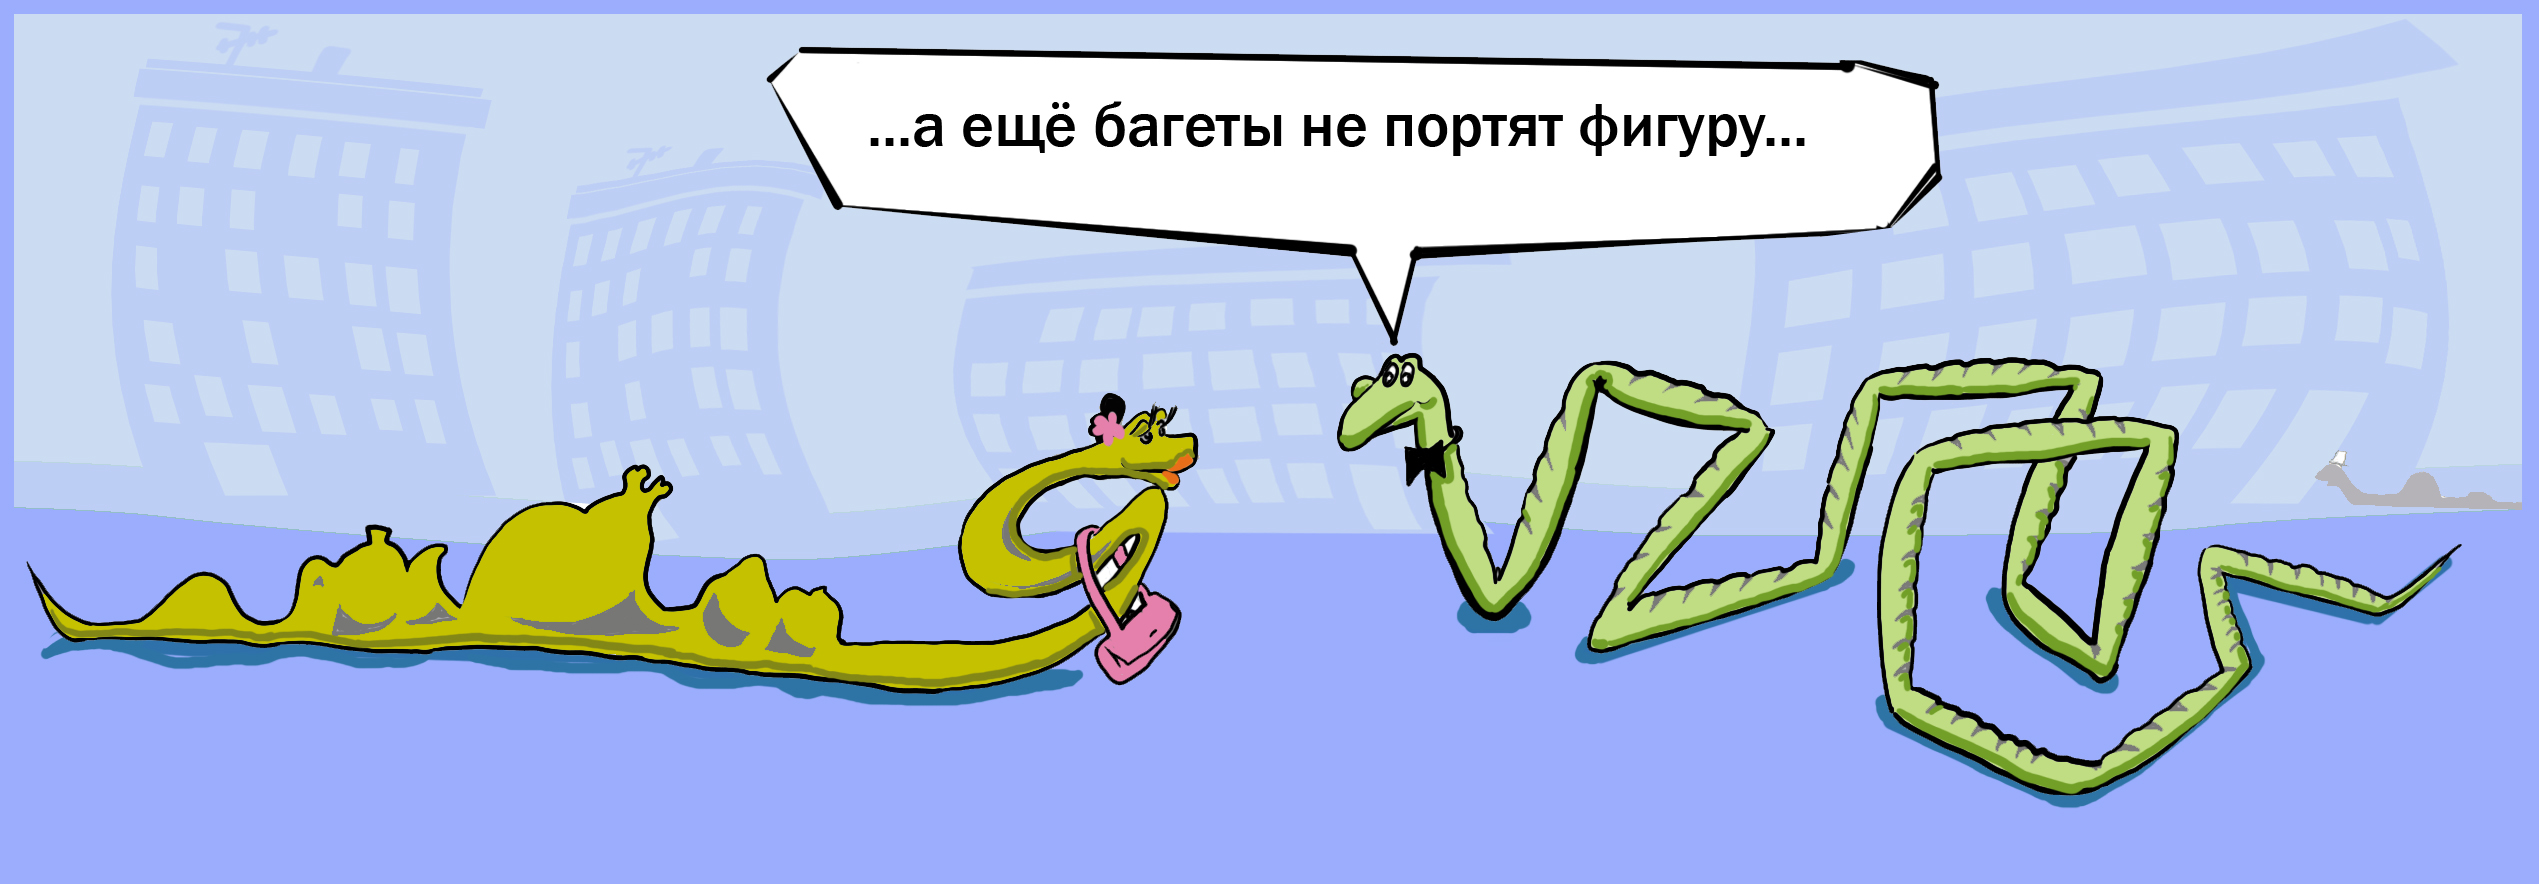
\includegraphics[width=17cm]{python_anatoliy.jpg}
  \caption{Удав Анатолий и Гюрза Леопольдина}
\end{figure*}


\begin{solution}
$\E(N)=e$.
\end{solution}


\item Жозеф Луи Франсуа Бертран подкидывает правильную монетку $n$ раз. Пафнутий Львович Чебышёв\footnote{Да, да, предпоследняя буква в окончании именно «ё»} подкидывает правильную монетку $(n+1)$ раз. Какова вероятность того, что у Пафнутия Львовича выпадет больше «орлов», чем у Жозефа Луи Франсуа?

\begin{solution}
Допустим, что после $n$ подбрасываний Пафнутий лидирует с вероятностью $p$. Тогда в силу симметрии задачи, вероятность равенства числа «орлов» после $n$ подбрасываний равна $1-2p$. Следовательно, вероятность победы Пафнутия равна $p+(1-2p)\frac{1}{2}=\frac{1}{2}$.
\end{solution}

\item Сломанный пульт.

Роберт Адлер нажимает на кнопку «Вкл/Выкл» на пульте дистанционного управления телевизором. Изначально телевизор включён. Батарейки у пульта сели, поэтому в первый раз кнопка срабатывает с вероятностью $1/2$. Далее вероятность срабатывания кнопки падает. Какова вероятность, что после 100 нажатий телевизор окажется включён?


\begin{solution}
Можно попробовать посчитать вероятности для нескольких первых нажатий и по индукции получить ответ $1/2$.
\end{solution}

\item Киллер

Правила игры «Киллер» просты. Игроки пишут на бумажках, как их зовут, и кладут бумажки в шляпу. Каждый тянет из шляпы имя своей первой жертвы. Если первой жертвой игрока является он сам, то он совершает «самоубийство» и дальше не играет\footnote{В некоторых вариантах правил, если игрок вытянул из шляпы своё имя, то он должен вытянуть другую бумажку.}. Чтобы убить жертву, надо остаться с ней наедине и сказать: «Ты убит!». Убийца забирает себе все бумажки, набранные убитым, и начинается охотиться за тем, за кем охотился убитый.  Побеждает тот, кто наберёт больше всех бумажек к концу игры. Заметим, что в «Киллере» каждый игрок оказывается втянут в одну из нескольких цепочек.

В «Киллера» играют 30 человек, из них 20 девушек.

\begin{enumerate}
\item Какова вероятность того, что в цепочке, начинающейся с Маши Сидоровой ровно 5 человек?
\item Какова вероятность того, что в цепочке, начинающейся с Маши Сидоровой ровно 5 девушек?
\item Какова вероятность того, что все девушки попадают в одну цепочку убийц и жертв?
\item Какова вероятность того, что все игроки попадают в общую цепочку?
\item Сколько в среднем цепочек в «Киллере»?
\item Сколько в среднем «самоубийц»?
\end{enumerate}

\begin{solution}

\end{solution}

\item  Ной Палмер Чепмэн\footnote{почтмейстер из Канастоты, вероятно, изобретатель игры «пятнашки»} рассыпал фишки для игры в пятнашки и расставляет их на поле в случайном порядке. Какова вероятность того, что он сможет решить получившуюся головоломку?

\begin{solution}
Легко экспериментально установить, что все фишки кроме двух последних можно поставить на свои места. Например, сначала выставляются $1$--$4$, затем $5$--$8$, затем $9$, $13$ и всё оставшееся кроме $14$ и $15$.  Один вариант не сводится к другому, так как любое движение в пятнашках не изменяет четность перестановки. Чётных и нечётных перестановок одинаковое количество, поэтому вероятность равна $1/2$.
\end{solution}

\item Задача о 100 заключенных

У ста узников тюрьмы есть последний шанс на спасение. В комнате стоит шкаф в котором сто занумерованных ящичков. Палач кладёт в каждый ящичек бумажку с номером ровно одного из заключенных в случайном порядке и задвигает все ящички. Узники заходят в комнату один за другим. Каждый узник может открыть любые 50 ящичков. После каждого узника все ящички задвигаются в исходное положение. Если каждый узник находит свой номер, то все узники будут помилованы. Если хотя бы один из узников не найдёт свой номер, то все будут казнены.

Узники могут предварительно договориться о стратегии.

\begin{enumerate}
\item Какова оптимальная стратегия?
\item Какую вероятность выигрыша она обеспечивает?
\end{enumerate}

\begin{solution}
Открыть ящичек со своим номером, далее открывать ящички с номером, написанным на вытащенной бумажке. Вероятность выигрыша, $1-(H_{100}-H_{50}) \approx 1- \ln 2$, где $H_n$ --- гармоническое число, $H_n=1+\frac{1}{2} + \frac{1}{3} + \ldots + \frac{1}{n}$.
\end{solution}

\item Андрей Абрикосов, Борис Бананов и Вова Виноградов играют одной командой в игру. В комнате три закрытых внешне неотличимых коробки: с абрикосами, бананами и виноградом. Общаться после начала игры они не могут, но могут заранее договориться о стратегии. Они заходят в комнату по очереди. Каждый из них может открыть две коробки по своему выбору. Перед следующим игроком коробки закрываются. Если Андрей откроет коробку абрикосами, Борис --- с бананами, а Вова --- с виноградом, то они выигрывают. Если хотя бы один из игроков не найдёт свой фрукт, то их команда проигрывает.

\begin{enumerate}
\item Какова оптимальная стратегия?

\item Какова вероятность выигрыша при использовании оптимальной стратегии?
\end{enumerate}


\begin{solution}
$2/3$
\end{solution}

\item Дед Мороз развешивает новогодние гирлянды. Аллея состоит из 1000 елок. Каждой гирляндой Дед Мороз соединяет две елки (не обязательно соседние). В результате Дед Мороз повесил 500 гирлянды и все елки оказались украшенными. Какова вероятность того, что существует хотя бы одна гирлянда, пересекающаяся с каждой из других?

Например, гирлянда 5-123 (гирлянда соединяющая 5-ую и 123-ю елки) пересекает гирлянду 37-78 и гирлянду 110-318.

\begin{solution}
$2/3$
\end{solution}


\item Птички на проводе

На телеграфный провод равномерно и независимо друг от друга садятся случайным образом  $n>>0$ птичек. Маляр-электрик Степан Грибоедов красит белой краской отрезок провода от каждой птички до ближайшей. Каждый участок провода оказывается в результате либо ни разу не покрашенным, либо покрашенным один или два раза.

Найдите среднюю длину непокрашенной части провода провода, части, покрашенной один раз и части, покрашенной два раза.

\begin{solution}
\url{http://www.cut-the-knot.org/Curriculum/Probability/BOW4.shtml}
\url{http://math.stackexchange.com/questions/227990/}
$2/18$, $5/18$, $11/18$
\end{solution}

\item В углу шахматный доски стоит конь. Мы перемещаем коня наугад, выбирая каждый допустимый ход равновероятно. Сколько в среднем пройдет ходов прежде чем он вернется в исходную клетку?

\begin{solution}
$168$
\end{solution}


\item Китайский ресторан

Каждый момент времени в китайский ресторан приходит новый посетитель.
Если сейчас в ресторане сидит $n$ человек, а за конкретным столиком сидит $b$ человек, то вероятность того, что новый посетитель присоединится к этому столику равна $\frac{b}{n+\theta}$. С вероятностью $\frac{\theta}{n+\theta}$ посетитель сядет за отдельный столик.

Каково ожидаемое число занятых столиков к моменту времени $n$?

\begin{solution}

\end{solution}

\item Правильную монетку подкидывают 1000 раз.
\begin{enumerate}
\item Найдите вероятность того, что ни разу не выпало два орла подряд
\item При чём тут числа Фибоначчи?
\end{enumerate}

\begin{solution}
$\frac{F_{1000}}{2^{1000}}$
\end{solution}

\item Двигаемся вверх-вниз или влево-вправо по фрактальному множеству.

\begin{enumerate}
\item Вероятность когда либо дойти до точки А?
\item Вероятность вернуться в начало координат?
\item Вероятность дойти до точки А раньше, чем до Б?
\end{enumerate}

\begin{solution}

\end{solution}

\item На заводе тортиков очень любят праздники! Если хотя бы у одного работника день рождения, то на заводе никто не работает, все празднуют и кушают тортики. Сколько работников нужно нанять, чтобы среднее количество рабочих дней в году было максимально?

\begin{solution}

\end{solution}

\item Аргонавты разного роста, $n$ человек, высадились на остров и идут по узкой тропинке друг за другом. Каждый аргонавт видит вперёд не далее спины более высокого аргонавта. Внезапно впереди самого первого аргонавта показалась Медуза Горгона, и все, кто видел её, $Z$ аргонавтов, обратились в камни.

\begin{enumerate}
\item Какова вероятность того, что в камень обратился последний аргонавт?
\item Найдите $\E(Z)$
\item Ясон идёт посреди аргонавтов. Пусть $X$ и $Y$ --- количество аргонавтов, обратившихся в камень до и после Ясона. Найдите $\Cov(X,Y)$.
\item Найдите $\Var(Z)$
\end{enumerate}


\begin{solution}
Разбиваем $Z$ в сумму индикаторов, $Z=Z_1 + \ldots + Z_n$. Замечаем, что $Z_k$ равно единице, если $k$-ый аргонавт выше чем, аргонавты $1$, $2$, \ldots $k-1$. Но максимум из первых $k$ величин равновероятно приходится на каждую из них, значит $\E(Z_k)=\P(Z_k=1)=1/k$. Отсюда $\E(Z)=\sum_{k=1}^n 1/k$. Замечаем, что $Z_i$ и $Z_j$ независимы. Следовательно, $\Cov(X,Y)=0$, а $\Var(Z)=\sum_{k=1}n \Var(Z_k)$.
\end{solution}


\item На планету Плюк в случайных точках садятся $n$ пепелацев. Радиосвязь между двумя точками на планете Плюк возможна, если центральный угол между этими двумя точками меньше $\pi/2$. 

\begin{enumerate}
\item Какова вероятность того, что из любой точки планеты можно связаться хотя бы с одним пепелацем?
\item Какова вероятность того, что при $n=3$ все три пепелаца смогут поддерживать связь друг с другом (необязательно напрямую, возможно через посредника)?
\end{enumerate}

\begin{solution}
$(\pi+2)/4\pi$
\end{solution}



\item красивые задачи из старой версии задачника...

\begin{comment}
\item Каждую минуту от конечной станции А отходит паровозик. Скорости паровозиков --- независимые, равномерные на $[0;1]$ случайные величины. Когда более быстрый паровозик догоняет более медленный, они едут вдвоём со скоростью более медленного.

...
Или про ракеты?
\end{comment}



\end{enumerate}

\section{Чуть менее классические задачи}

\begin{enumerate}
\item Стрелок попадает по мишени с вероятностью 0.3. Какова вероятность того, что до третьего промаха у него будет 5 выстрелов?

\item Расстояние от пункта A до B автобус проходит за 2 мин, а пешеход — за 20 мин. Интервал движения автобусов 30 мин. Вы подходите в случайный момент времени к пункту A и отправляетесь в B пешком.

\begin{enumerate}
\item Какова вероятность того, что в пути Вас догонит очередной автобус?
\item Сколько в среднем времени Вы будете добираться, если проходящий мимо автобус обязательно Вас подбирает?
\end{enumerate}

% 18/30, примерно 14 минут


\item Для простоты предположим, что ген карих глаз доминирует ген синих. Т.е. у носителя пары bb глаза синие, а у носителя пар BB и Bb --- карие. У диплоидных
организмов \marginnote{А мы тут все диплоидные :)} одна аллель наследуется от папы, а одна --- от мамы. В семье у кареглазых родителей два сына --- кареглазый и
синеглазый. Кареглазый женился на синеглазой девушке. Какова
вероятность рождения у них синеглазого ребенка?


\item Задача о полосе невезения

За неделю Аннушка семь раз пролила масло. Какова вероятность того, что она проливала масло каждый день?



\end{enumerate}


\begin{comment}
\section{Черновые размышления :)}

сколько теории игр включать?

менее канонические задачи ??? ()




Методы: ! это отдельный документ!!!

Первый шаг

Разложение в сумму --- Разделяй и властвуй

Большая сила о-малых

Матрешки --- (условное математическое ожидание)

Холмс, это невероятно! (Вероятностная интерпретация)

Как сварить мартингал (теорема Дуба)

Свернулся колечком (задачи на равномерное на отрезке)


Сюжеты: ????

Пуассоновский поток

Броуновское движение



\end{comment}



\section{Источники мудрости}

Источники мудрости, кои автор подборки постарался не замутить. Смело направляйте к ним верблюдов своего любопытства!

\nocite{*}

\printbibliography


\end{document}
